\documentclass[10pt,a4paper,notitlepage,twocolumn,twoside]{article}

\usepackage[utf8]{inputenc}
\usepackage[a4paper,left=0.5in,right=0.5in,top=1.0in,bottom=1.0in]{geometry}
\usepackage{hyperref}
\usepackage{graphicx}
\usepackage[caption=false,font=footnotesize]{subfig}
\usepackage{array}
\usepackage{amsmath,amssymb,amsfonts}
\usepackage{mathtools}
\usepackage[ruled,vlined,linesnumbered,commentsnumbered]{algorithm2e}
\usepackage{endnotes}
\usepackage{fancyhdr}

\DeclareMathOperator{\sign}{sign}
\DeclareMathOperator{\ssin}{s}
\DeclareMathOperator{\scos}{c}
\DeclareMathOperator{\atan2}{atan2}
\DeclareMathOperator{\satan}{atan}

\renewcommand{\footnoterule}{%
  \kern -3pt
  \hrule width \columnwidth height 0.1pt
  \kern 4.5pt
}

\pagestyle{myheadings}
%\fancyhf{}
\markboth{Ricardo B. Sousa and Rui M. Coutinho}{Summarized Report of the Final Project: Bowling Robot Arm}



%%%%%%%%%%%%%%%%%%%% ARTICLE INFORMATION

\title{\Large Ph.D in ECE @ FEUP: Robotic Manipulators 2021/2022\\
\LARGE Summarized Report of the Final Project: Bowling Robot Arm%
\thanks{%
\noindent Ricardo B. Sousa\textsuperscript{1, 2}

\noindent \href{mailto:up201503004@edu.fe.up.pt}{up201503004@edu.fe.up.pt}

\vspace{0.5em}
\noindent Rui M. Coutinho\textsuperscript{1}

\noindent \href{mailto:up201503006@edu.fe.up.pt}{up201503006@edu.fe.up.pt}

\vspace{1em}
\noindent \textsuperscript{1} Faculty of Engineering of the University of Porto, Electrical Engineering Department, Porto, 4200-465 Porto, Portugal

\noindent \textsuperscript{2} INESC TEC -- Institute for Systems and Computer Engineering, Technology and Science, CRIIS -- Centre for Robotics in Industry and Intelligent Systems, Porto, 4200-465 Porto, Portugal
\vspace{-3pt}\rule{\columnwidth}{0.1pt}\vspace{4.5pt}
}}
\author{%
Ricardo B. Sousa
\href{https://orcid.org/0000-0003-4537-5095}{
\includegraphics[width=1em]{orcid.pdf}}%
\and%
Rui M. Coutinho%
%\href{https://orcid.org/}{
\includegraphics[width=1em]{orcid.pdf}}%
}
\date{January 2022}



%%%%%%%%%%%%%%%%%%%% ARTICLE BODY

\begin{document}

\maketitle

\section{Introduction}
\label{sec:intro}

This work represents the final project developed in the scope of the course Robotic Manipulators (RM) of the doctoral program in Electrical and Computers Engineering (ECE) at the Faculty of Engineering of the University of Porto (FEUP). The project consists in developing an automated system based on a robot manipulator for playing bowling. The bowling game and the robot manipulator are simulated in the SimTwo~\cite{simtwo:article,simtwo:github}. As for the application to interact with the user, it is developed in Lazarus, a cross-platform IDE compatible with Delphi. All the code is available in a GitHub repository\footnote{\url{https://github.com/sousarbarb/pdeec-rm}}.

The rest of the report is organized as follows. Section~\ref{sec:robot} presents the simulated robot manipulator. Section~\ref{sec:scene} presents the bowling scene developed in SimTwo. Section~\ref{sec:kinematics} formulates the forward and inverse kinematics of the robot. Section~\ref{sec:app} explains the application developed in Lazarus. Section~\ref{sec:results} presents the experimental results obtained in this work. Lastly, Section~\ref{sec:conclusions} presents the conclusions.

\section{Robot Manipulator}
\label{sec:robot}

A robot manipulator is required in this work to be able to pick the ball and throw it in the direction of the bowling pins. The manipulator used in SimTwo is illustrated in figure~\ref{fig:robot}, in which the blue axes help identify the 7 Degrees of Freedom (DoF) of the robot. Six of them can be viewed as an independent articulated/anthropomorphic manipulator represented by a RRR (the first three revolute joints) kinematic arrangement followed by a spherical wrist (the other 3 revolute joints represented in figure~\ref{fig:robot})~\cite{book:spong:2005}. The other DoF simulates the anthropomorphic manipulator attached to a prismatic joint for adding kinematic redundancy.

\begin{figure}[!t]
  \centering
  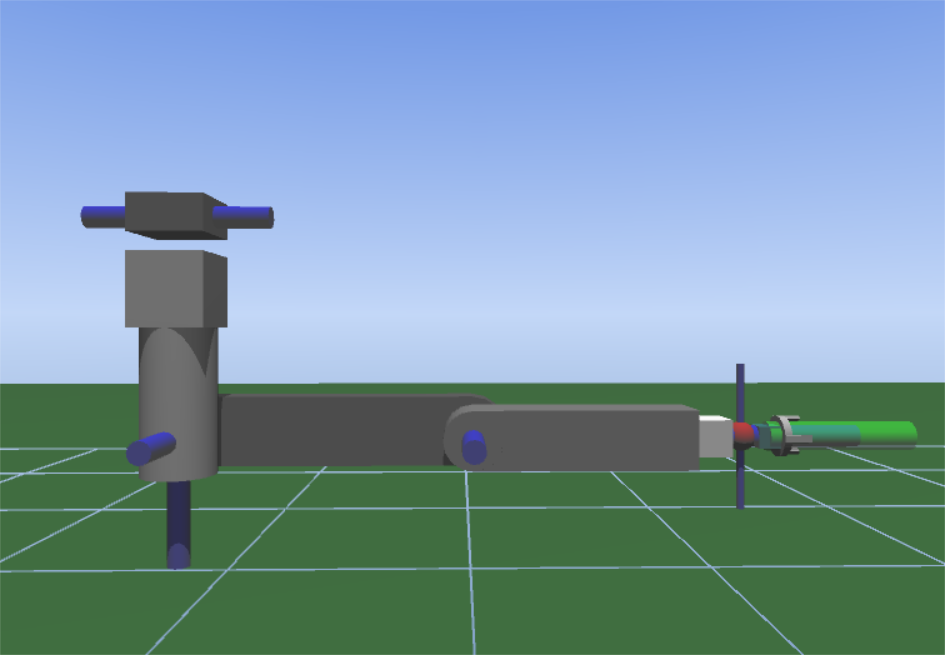
\includegraphics[width=0.45\textwidth]{images/manipulator-7dof.png}
  \caption{Robot manipulator used in SimTwo with 7 Degrees of Freedom (DoF)}
  \label{fig:robot}
\end{figure}

The main reason to choose the anthropomorphic kinematic arrangement is due to its similar behavior to a human arm, given the goal of simulating a bowling game. Furthermore, the use of the spherical wrist allows an independent formulation of the robot's inverse kinematics in terms of position and orientation, as presented in Section~\ref{sec:kinematics}~\cite{book:spong:2005}.

As for picking the bowling ball, the simulated robot has a magnetic actuator in its tool. The ball is modified to have ferromagnetic properties. These properties allow the magnetic actuator to grab the bowling ball. Although the goal would be attracting all magnetic objects around the actuator, SimTwo simulates the actuator only within a circumscribed cylinder.

In terms of our contribution for developing this arm in SimTwo, the original version only had 6 DoF equivalent to an anthropomorphic manipulator. We added the prismatic joint for having more flexibility to pick the ball and throw it. Furthermore, we adapted the wrist size to be compatible with the bowling ball dimensions. Although we tried to reduce the overall size of the robot for scale purposes, the simulation became unstable leading to not changing the original scale. So, we only changed the wrist dimensions. Another modification is the friction added to the three anthropomorphic joints of the robot. However, the current version is not fully stable and needs further improvements in future work.

\section{Bowling Scene}
\label{sec:scene}

All the dimensions of the bowling scene developed in SimTwo are the same ones available in Dimensions -- Database of Dimensioned Drawings\footnote{\url{https://www.dimensions.com/element/bowling-lane}} \footnote{\url{https://www.dimensions.com/element/ten-pin-pin-deck}}. These dimensions follow the official equipment specifications and certifications manual\footnote{\url{http://usbcongress.http.internapcdn.net/usbcongress/bowl/equipandspecs/pdfs/ESManual.pdf}} from the United States Bowling Congress (USBC). The SimTwo bowling scene developed by us is illustrated in figure~\ref{fig:scene}. Relative to the USBC bowling official dimensions, we apply a scale reduction factor for avoiding the bowling lane to exceed the available space in SimTwo's scene.

\begin{figure}[!t]
  \centering
  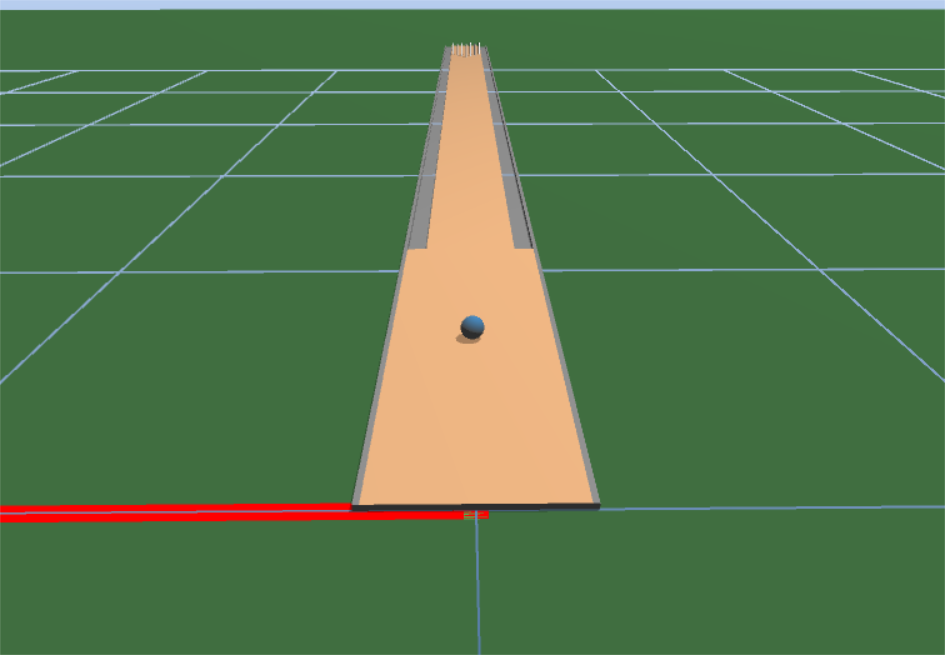
\includegraphics[width=0.475\textwidth]{images/bowling-scene.png}
  \caption{Bowling simulation scene developed in SimTwo}
  \label{fig:scene}
\end{figure}

Another detail is the simulation of the 10-pin bowling deck. Two different versions are illustrated in Figure~\ref{fig:10-pin}. Given that SimTwo only has available simple collision models (e.g., cuboid, cylinder, or sphere), these versions are only composed of cylinders to try to model a 10-pin deck bowling pin. The first version, Figure~\ref{fig:10-pin:real}, is the most realistic one in which the radius of the two cylinders corresponds to the base and maximum outer diameters of a 10-pin deck bowling pin. The other version, Figure~\ref{fig:10-pin:fast}, only models the base diameter of the bowling pin. Although the version in Figure~\ref{fig:10-pin:real} is more realistic, the simulation runs on approximately 12.9fps with no motion. In contrast, but using the same conditions, Figure~\ref{fig:10-pin:fast}'s version achieves 20.8fps. The main reason is that the first version requires the definition of a \texttt{robot} tag for each pin, while in the second version all pins are treated with the \texttt{things} tag being more light for the simulation. Note that the fps values should be interpreted relative to each other and not in terms of the absolute values due to being dependent on the computer performance. Even so, we chose the lighter version in terms of fps for having a fluid simulation and interaction with the user.

\begin{figure}[!t]
  \centering
  \subfloat[][]{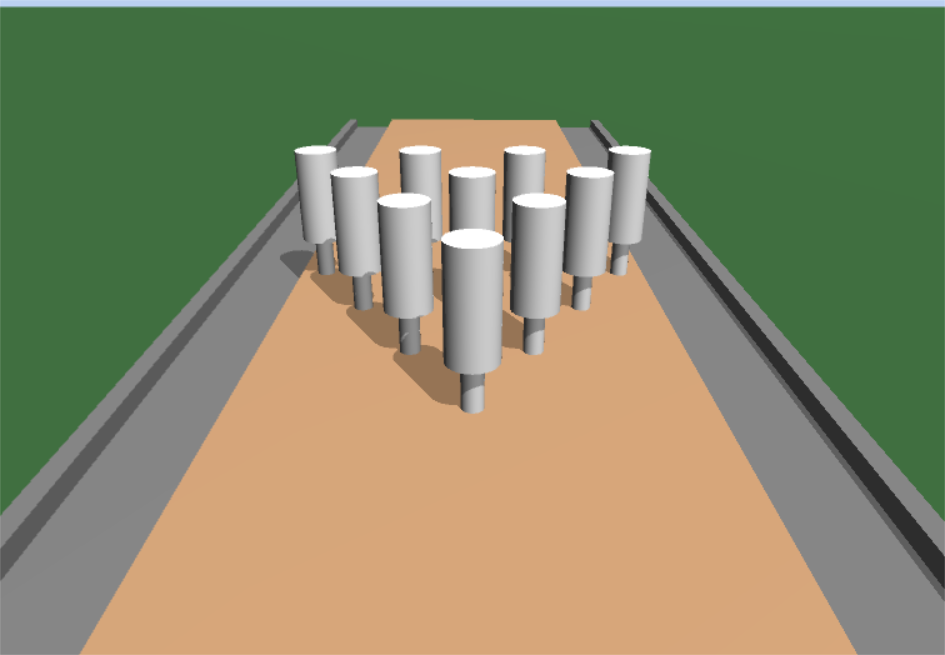
\includegraphics[width=0.24\textwidth]{images/10-pin-set_realistic.png}%
  \label{fig:10-pin:real}}
  \hfill
  \subfloat[][]{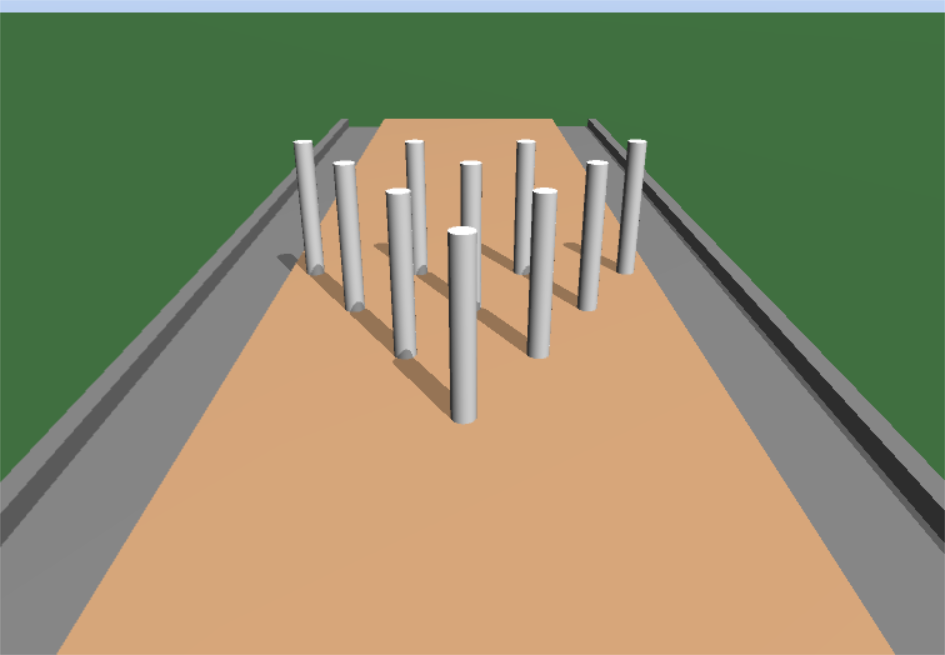
\includegraphics[width=0.24\textwidth]{images/10-pin-set_fast.png}%
  \label{fig:10-pin:fast}}
  \caption{Simulated 10-pin bowling pin deck: (a) more realistic version; (b) simple and light version}
  \label{fig:10-pin}
\end{figure}

\section{Kinematics}
\label{sec:kinematics}

In this section, the forward and inverse kinematics are formulated for the robot manipulator used in this work. These kinematics are based on the ones presented in~\cite{book:spong:2005}. First, the kinematics are presented for the anthropomorphic arm. Then, the transformations between the world and the robot's base coordinate frame ($\{X^W,Y^W,Z^W\}$ and $\{X^0,Y^0,Z^0\}$, respectively) are explained in the context of setting the desired pose and orientation for the robot's tool.

\subsection{Anthropomorphic robot manipulator}

\subsubsection{Forward kinematics}

Following the Denavit-Hartenberg (DH) convention, the obtained coordinates frames for the anthropomorphic robot arm are the ones illustrated in Figure~\ref{fig:kinematics:frames}. These frames originate the DH parameters presented in Table~\ref{tab:kinematics:dh}.

\begin{figure*}[!t]
  \centering
  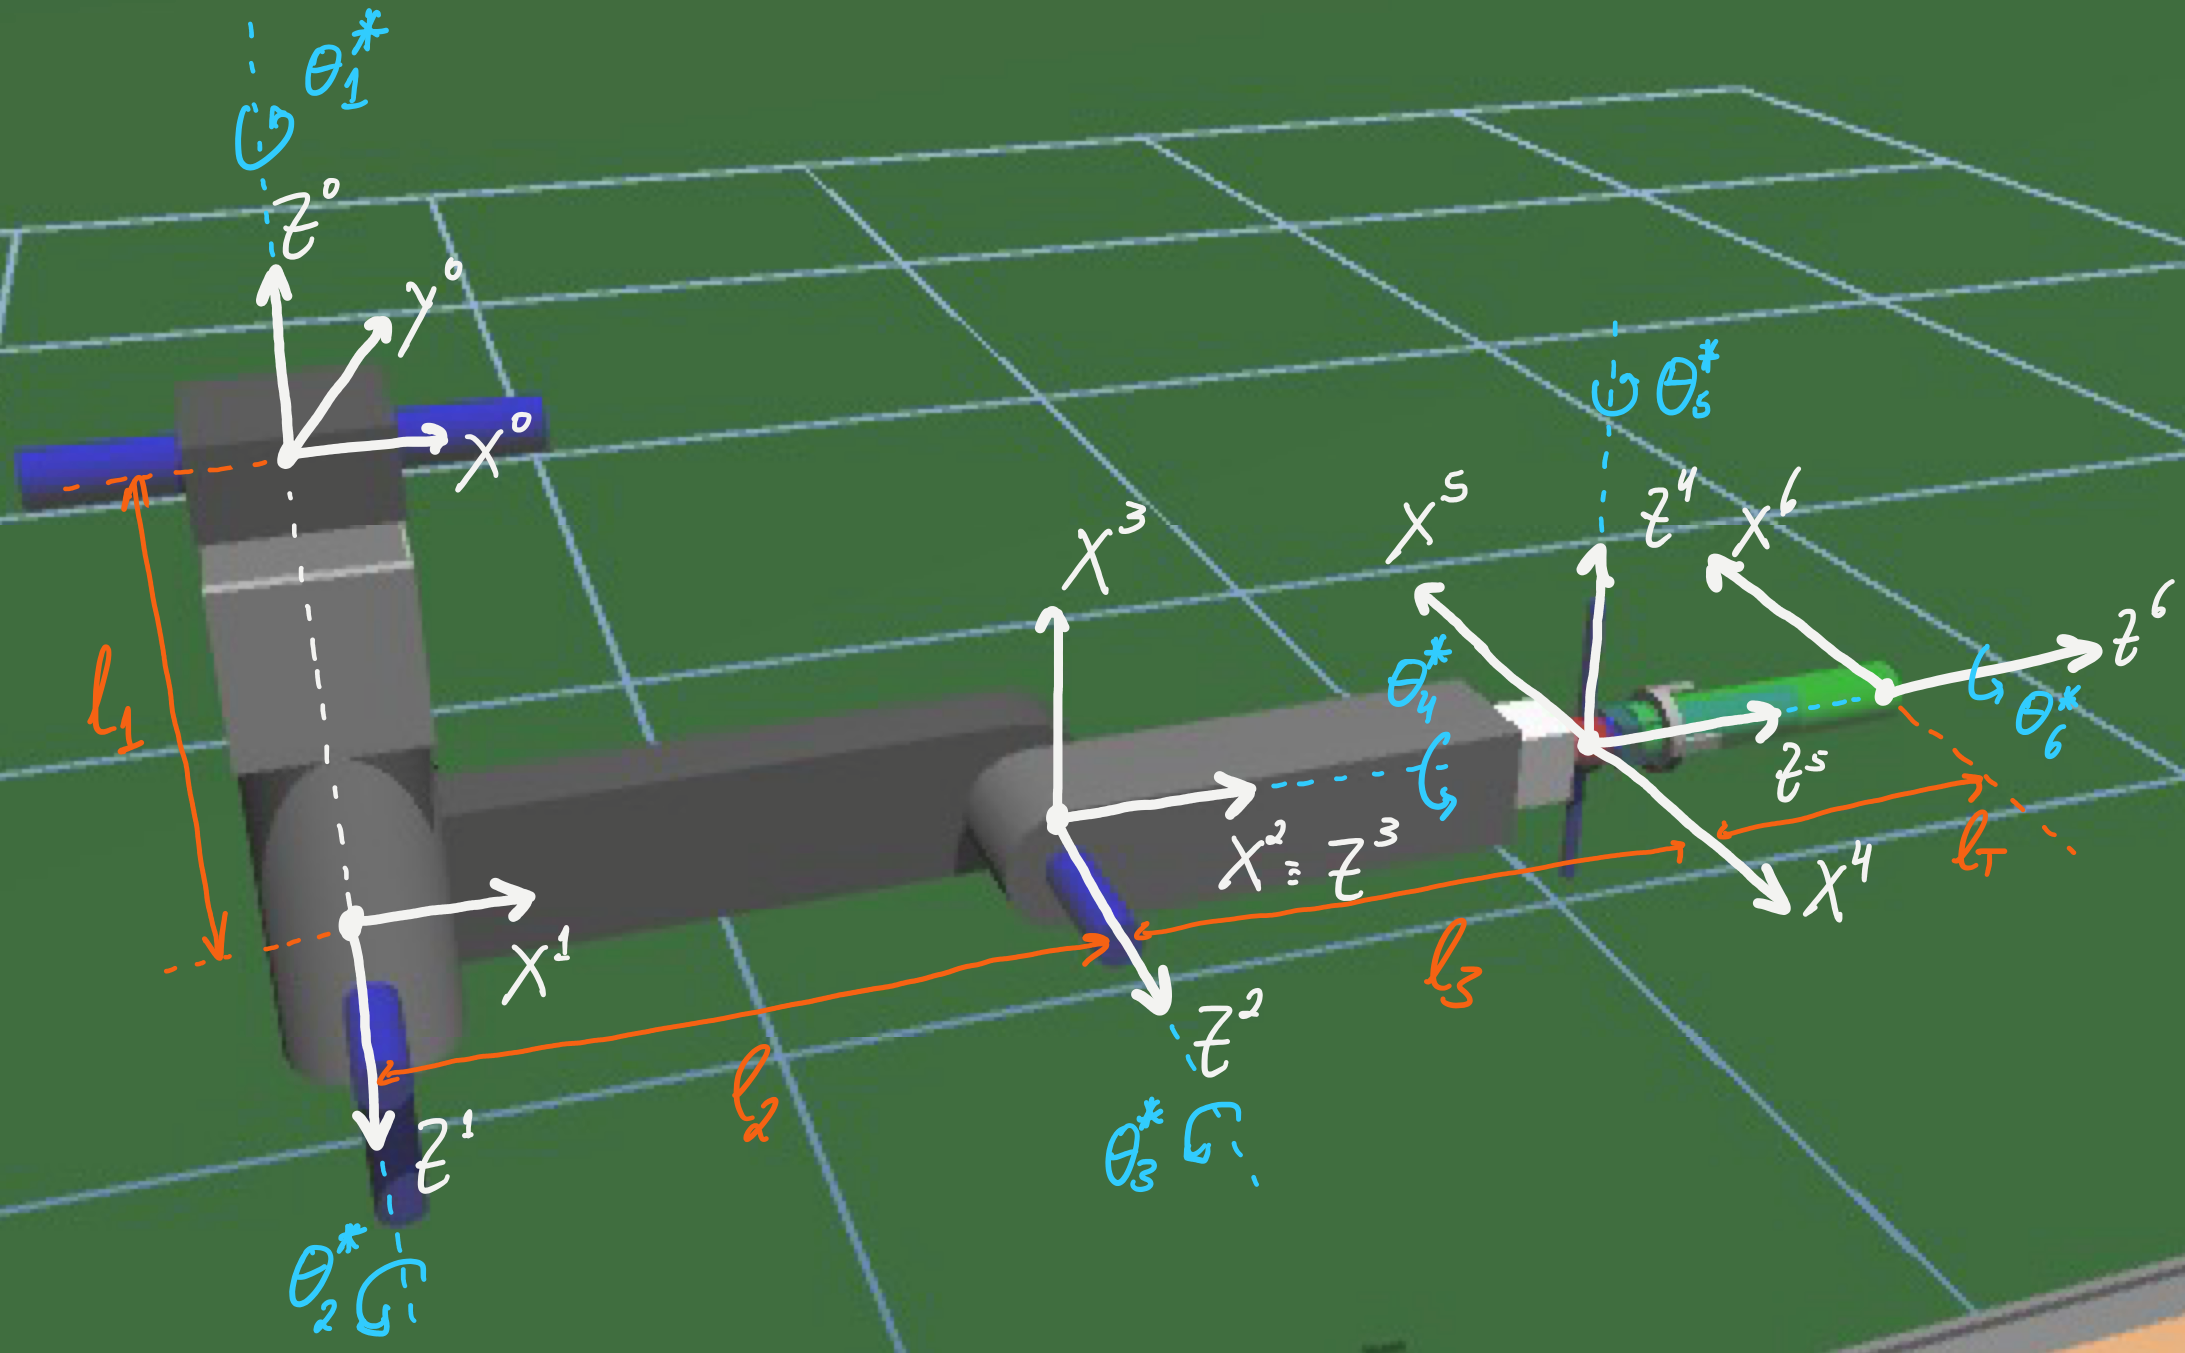
\includegraphics[width=0.8\textwidth]{images/kinematics-forward_v2.png}
  \caption{Coordinate frames of the anthropomorphic robot arm accordingly to the Denavit-Hartenberg (DH) convention}
  \label{fig:kinematics:frames}
\end{figure*}

\begin{table}[!t]
  \renewcommand{\arraystretch}{1.25}
  \setlength{\tabcolsep}{2pt}
  \caption{Denavit-Hartenberg (DH) parameters of the anthropomorphic robot arm}
  \label{tab:kinematics:dh}
  \centering
  \begin{tabular}{c | c c c c}

\hline
\textbf{i} & \textbf{Rot.\textsubscript{Z}} ($\theta_i$) & \textbf{Trans.\textsubscript{Z}} ($d_i$) & \textbf{Trans.\textsubscript{X}} ($a_i$) & \textbf{Rot.\textsubscript{X}} ($\alpha_i$)\\
\hline
1 & $\theta_1^*$             & $-l_1$ & 0 m   & 90º\\
2 & $\theta_2^*$             & 0 m    & $l_2$ & 0º\\
3 & $\theta_3^*+90\text{º}$  & 0 m    & 0 m   & 90º\\
4 & $\theta_4^*+90\text{º}$  & $l_3$  & 0 m   & 90º\\
5 & $\theta_5^*+180\text{º}$ & 0 m    & 0 m   & 90º\\
6 & $\theta_6^*$             & $l_T$  & 0 m   & 0º\\
\hline

  \end{tabular}
\end{table}

Equation~\ref{eq:kinematics:dh} formulates the homogeneous transformation dependent on the DH parameters of the $i$ coordinate frame: joint angle ($\theta_i$, rotation around z-axis), link offset ($d_i$, translation on the z-axis), link length ($a_i$, translation on the x-axis), and link twist ($\alpha_i$, rotation around x-axis). Multiplying the 6 homogeneous transformation matrices equivalent to each entry $i$ in Table~\ref{tab:kinematics:dh} and as shown in the Equation~\ref{eq:kinematics:forward}, we obtain the forward kinematics for the anthropomorphic arm that we implemented.

\begin{equation}\label{eq:kinematics:dh}
A_i = \begin{bmatrix}
\scos_{\theta_i} & -\ssin_{\theta_i}\scos_{\alpha_i} &  \ssin_{\theta_i}\ssin_{\alpha_i} & a_i \scos_{\theta_i}\\
\ssin_{\theta_i} &  \scos_{\theta_i}\scos_{\alpha_i} & -\scos_{\theta_i}\ssin_{\alpha_i} & a_i \ssin_{\theta_i}\\
0                &  \ssin_{\alpha_i}                 &  \scos_{\alpha_i}                 & d_i \\
0                &  0                                &  0                                & 1\\
\end{bmatrix}
\end{equation}

\begin{equation}\label{eq:kinematics:forward}
H_6^0 = A_1 \cdot A_2 \cdot A_3 \cdot A_4 \cdot A_5 \cdot A_6
\end{equation}

\subsubsection{Inverse kinematics}

In terms of inverse kinematics, as already stated in Section~\ref{sec:robot}, one advantage of using a spherical wrist is the decoupling of position and orientation inverse kinematics. Consequently, we can formulate the inverse kinematics for the wrist position ($o_c^0$) dependent on the desired position and orientation for the arm's tool ($o$ and $R$, respectively) while only using the first 3 revolute joints ($\theta_1$, $\theta_2$, and $\theta_3$). This formulation is equivalent to Equation~\ref{eq:kinematics:inverse:decoupling:position}. Then, the tool's orientation is achieved by computing the orientation $R_6^3$ only dependent on the last three revolute joints ($\theta_4$, $\theta_5$, and $\theta_6$) equivalent to the ones of the spherical wrist, as presented in Equation~\ref{eq:kinematics:inverse:decoupling:orientation}.

\begin{equation}\label{eq:kinematics:inverse:decoupling:position}
o_c^0 = \begin{bmatrix}
x_c\\y_c\\z_c\\
\end{bmatrix} = o - R \cdot \begin{bmatrix}
0\\0\\l_T
\end{bmatrix} = \begin{bmatrix}
x\\y\\z\\
\end{bmatrix} - R \cdot \begin{bmatrix}
0\\0\\l_T
\end{bmatrix}
\end{equation}

\begin{equation}\label{eq:kinematics:inverse:decoupling:orientation}
R_6^3 = \left(R_3^0\right)^T R
\end{equation}

Furthermore, first, we need to compute the reference values required for achieving $o_c^0$. Joint 1 ($\theta_1$) is computed by Equation~\ref{eq:kinematics:inverse:q1}. As shown in the equation, there are 2 possible solutions for this joint. We opted for the first one. A special case occurs when both $x_c$ and $y_c$ are 0 equivalent to the wrist being on the rotation axis of the joint 1. Given the infinite number of solutions for this case, we maintain the last reference value for $\theta_1$.

\begin{equation}\label{eq:kinematics:inverse:q1}
\theta_1 = \atan2\left(y_c,x_c\right) \text{ or } \pi + \atan2\left(y_c,x_c\right)
\end{equation}

Next, Equations~\ref{eq:kinematics:inverse:s}, \ref{eq:kinematics:inverse:r}, and \ref{eq:kinematics:inverse:d} compute auxiliary variables ($s$, $r$, and $D$). These variables are used to compute the value of joint 3 ($\theta_3$), as formulated in Equation~\ref{eq:kinematics:inverse:q2}. Two possible solutions exist for the possibility of having the elbow up or elbow down (minus or plus in the equation, respectively). Our implementation considers both solutions depending on the user setting elbow up or down.

\begin{equation}\label{eq:kinematics:inverse:s}
s = z_c - l_1
\end{equation}

\begin{equation}\label{eq:kinematics:inverse:r}
r = \sqrt{x_c^2 + y_c^2}
\end{equation}

\begin{equation}\label{eq:kinematics:inverse:d}
\scos_{\theta_3} = \frac{s^2+r^2-l_2^2-l_3^2}{2l_2l_3} := D
\end{equation}

\begin{equation}\label{eq:kinematics:inverse:q2}
\theta_3 = \atan2\left(\pm\sqrt{1-D^2},D\right)
\end{equation}

Joint 2 ($\theta_2$) is computed depending on the auxiliary variables ($s$, $r$, and $D$), links' lengths ($l_2$ and $l_3$, also illustrated in Figure~\ref{fig:kinematics:frames}), and the value of the joint 2 itself. This computation is formulated in Equation~\ref{eq:kinematics:inverse:q3}.

\begin{equation}\label{eq:kinematics:inverse:q3}
\theta_2 = \atan2\left(s,r\right) - \atan2\left(l_3\ssin_{\theta_3},l_2+l_3\scos_{\theta_3}\right)
\end{equation}

As for the inverse kinematics for the wrist's orientation ($R_6^3$), Equation~\ref{eq:kinematics:inverse:r63} formulates the matrix $R_6^3$ dependent on the values of the joints 4, 5, and 6 ($\theta_4$, $\theta_5$, and $\theta_6$, respectively). This equation was obtained using symbolic math in Matlab (scripts also available in our GitHub repository referred in Section~\ref{sec:intro}). Then, the inverse kinematics for $R_6^3$ are formulated as in the Algorithm~\ref{a:inverse-kinematics}.

\begin{equation}\label{eq:kinematics:inverse:r63}
\begin{aligned}
R_6^3 & = \begin{bmatrix}
r_{11} & r_{12} & r_{13}\\
r_{21} & r_{22} & r_{23}\\
r_{31} & r_{32} & r_{33}\\
\end{bmatrix} =\\
& = \begin{bsmallmatrix}
\scos_{\theta_4}\ssin_{\theta_6} + \ssin_{\theta_4}\scos_{\theta_5}\scos_{\theta_6} & \scos_{\theta_4}\scos_{\theta_6} - \ssin_{\theta_4}\scos_{\theta_5}\ssin_{\theta_6} & \ssin_{\theta_4}\ssin_{\theta_5}\\
\ssin_{\theta_4}\ssin_{\theta_6} - \scos_{\theta_4}\scos_{\theta_5}\scos_{\theta_6} & \ssin_{\theta_4}\scos_{\theta_6} + \scos_{\theta_4}\scos_{\theta_5}\ssin_{\theta_6} & -\scos_{\theta_4}\ssin_{\theta_5}\\
-\ssin_{\theta_6}\scos_{\theta_6} & \ssin_{\theta_6}\ssin_{\theta_6} & \scos_{\theta_5}
\end{bsmallmatrix}
\end{aligned}
\end{equation}

\begin{algorithm}[t!]
\DontPrintSemicolon
\SetAlgoLined\SetKwData{Left}{left}\SetKwData{This}{this}\SetKwData{Up}{up}
\SetKwFunction{Union}{Union}\SetKwFunction{FindCompress}{FindCompress}
\SetKwInOut{Input}{input}\SetKwInOut{Output}{output}

\Input{$R_6^3$}
\Output{$\theta_4$,$\theta_5$,$\theta_6$}

\BlankLine

$\theta_5=\atan2\left(\pm\sqrt{1-r_{33}^2},r_{33}\right)$\;
\uIf{$\left(r_{13}\neq0\right)$ AND $\left(r_{23}\neq0\right)\Leftrightarrow\ssin_{\theta_5}\neq0$, $\scos_{\theta_5}=0$}{
  $\theta_4=\atan2\left(r_{13},-r_{23}\right)$\;
  $\theta_6=\atan2\left(r_{32},-r_{31}\right)$\;
}
\Else{
  $\theta_4=0$\;
  \uIf{$r_{33}\Leftrightarrow\scos_{\theta_5}=1$}{
    \tcc{$\theta_4+\theta_6=\atan2\left(r_{11},r_{12}\right)$}
    $\theta_6=\atan2\left(r_{11},r_{12}\right)$\;
  }
  \Else{
    \tcc{$\theta_4-\theta_6=\atan2\left(-r_{11},r_{12}\right)$}
    $\theta_6=-\atan2\left(-r_{11},r_{12}\right)$\;
  }
}

\caption{Inverse kinematics for the orientation of the wrist}
\label{a:inverse-kinematics}
\end{algorithm}

In the implementation, there is still a bug to resolve in the computation of $\theta_1$ depending on which quadrant the desired pose is found. Even though we could not solve it on time of delivery, our implementation is still stable to play the simulated bowling game, as shown in Section~\ref{sec:results}.

\subsection{World -- robot base coordinate frames}

The coordinates of the bowling ball are sent to our application in the world coordinate frame. For having consistency between the kinematics formulated in the previous subsection and the ball position, we convert the ball position from the world to the anthropomorphic arm's base coordinate frame ($\{X^W,Y^W,Z^W\}$ and $\{X^0,Y^0,Z^0\}$, respectively). The transformation between these two frames is formulated in the following two equations:

\begin{equation}
H_0^W = \begin{bmatrix}
R_0^W & T_0^W\\
0 & 1\\
\end{bmatrix} =
\begin{bmatrix}
1 & 0 & 0 & 0.57125 + q_0\\
0 & 1 & 0 & 0.00\\
0 & 0 & 1 & 1.15\\
0 & 0 & 0 & 1\\
\end{bmatrix}
\end{equation}

\begin{equation}
H_W^0 = \begin{bmatrix}
{R_0^W}^T & -{R_0^W}^T \cdot T_0^W\\
0 & 1\\
\end{bmatrix}
\end{equation}

\noindent in which $q_0$ is the current value of the prismatic joint. Thus, the homogeneous matrix $H_W^0$ is used to convert the ball coordinates to the robot's base coordinate frame.

\section{Application}
\label{sec:app}

As for the application to communicate with SimTwo, it was developed in Lazarus that is a cross-platform IDE compatible with Delphi. A preview of the main window is shown in Figure~\ref{fig:app} on the application's simulation tab, with which the user must interact for throwing the bowling ball.

\begin{figure*}[!t]
  \centering
  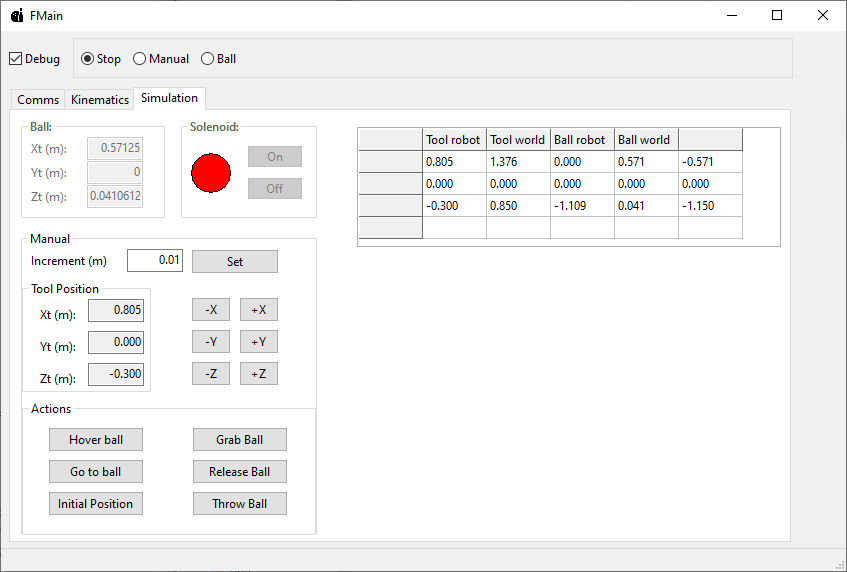
\includegraphics[width=0.7\textwidth]{images/app.png}
  \caption{Lazarus-based application for playing the simulated bowling game}
  \label{fig:app}
\end{figure*}

The application communicates with SimTwo over a UDP connection. The simulator sends the current joints' position and velocity and the ball position. As for the application, the position reference for the joints and the desired state for the magnetic actuator is sent over the UDP connection. We focus on playing the simulated bowling game instead of improving the original control scheme (PID-based controllers for the joints' reference position). This approach was chosen for having the assurance of having a first stable version. Although the several improvements can be made to our application and specially on the control side, it is at least stable for the purpose of playing the bowling game with the simulated robot manipulator.

For playing the bowling game, you must choose the Ball control mode in the application. The ball position can be reset in the SimTwo sheet. Then, the following steps are required for playing (wait for the robot to reach its steady-state between steps):

\begin{enumerate}
\item Hover ball
\item Go to ball
\item Grab ball
\item Adjust the y-axis position by clicking on \texttt{+Y} or \texttt{-Y}
\item Throw ball
\end{enumerate}

\section{Results}
\label{sec:results}

The experimental results from this work are presented in a YouTube video\footnote{\url{https://www.youtube.com/watch?v=lY1BQs15W1s}}. This video shows how to execute the Lazarus-based application and the simulation environment for you to experiment later.

In terms of throwing the bowling ball, it is clear that our implementation is capable of doing that. However, the video also shows the main disadvantage of our implementation: the control scheme of the joints. Even though we only actuate the prismatic joint when throwing the ball, the other joints are affected by that actuation. The reason is due to the original PID-based controlling scheme assuming independent joint control. The inertia from throwing the ball grasped by the arm's tool leads to disturbances on all the joints. A possible solution would be multivariable control using a state-space control scheme. This control scheme could consider the problem of inverse dynamics for diminishing the influence of the arm's mass and inertia on motion, even though the ball would still be treated as a disturbance. However, this approach was not implemented and was left out for future work.

Finally, the possibility of adjusting in \texttt{+Y} or \texttt{-Y} for throwing the ball resulted in the expected result of changing the final trajectory of the ball. 

\section{Conclusions and Future Work}
\label{sec:conclusions}

In conclusion, this work can simulate a bowling game, even though we had problems in terms of stabilizing the simulation and related to the joint's control scheme. All the dimensions of a bowling lane can be easily scaled for modeling a real implementation of a downsized version. Moreover, the application developed in Lazarus is modular in the terms of separating the GUI from the kinematics implementation of the robot facilitating further improvements to this work.

As for future work, the simulation must be modified to be more stable. The robot arm could also be downsized to allow a real implementation of the whole system. In terms of control, the control scheme can be changed to velocity-based control to allow the definition of the throwing velocity. Lastly, the kinematic redundancy of the 7 DoF robot manipulator can be useful to leverage. One possibility would be the computation of the singular valuables of the anthropomorphic's Jacobian matrix and evaluating the inverse kinematics solution that leads to the highest of the smallest singular values. Another possibility would be implementing an optimization-based approach to evaluate the joint space solutions that best suit a trajectory given by the user considering different cost functions.

\bibliographystyle{unsrt}
\bibliography{references.bib}

%\theendnotes

\end{document}
